\chapter{Requirements Specifications}

\section{Functional Requirements}
The following table outlines the main functional requirements for Nexora:

\begin{itemize}
    \item \textbf{User Authentication \& Role Management}
    \begin{itemize}
        \item FR-01: The system allows vendors, customers, and admins to create accounts and log in securely.
        \item FR-02: The system provides role-based access, restricting actions based on user type.
        \item FR-03: The system allows users to reset passwords through email verification.
    \end{itemize}
    \item \textbf{Vendor Management}
    \begin{itemize}
        \item FR-04: The system allows vendors to register, update, and delete their profiles.
        \item FR-05: The system enables vendors to add, edit, and remove products.
        \item FR-06: The system allows vendors to view and manage orders.
        \item FR-07: The system generates sales reports for vendors based on transactions.
    \end{itemize}
    \item \textbf{Product Management}
    \begin{itemize}
        \item FR-08: The system allows vendors to add products with images, descriptions, and prices.
        \item FR-09: The system enables customers to search for products using filters such as category, price, and rating.
        \item FR-10: The system displays product availability based on vendor stock levels.
    \end{itemize}
    \item \textbf{Shopping Cart \& Checkout}
    \begin{itemize}
        \item FR-11: The system allows customers to add, update, and remove items from the shopping cart.
        \item FR-12: The system displays the total price, including applicable taxes or discounts.
        \item FR-13: The system allows customers to proceed to check out and make payments securely.
        \item FR-14: The system generates a unique order ID for every purchase.
    \end{itemize}
    \item \textbf{Order Processing \& Tracking}
    \begin{itemize}
        \item FR-15: The system allows customers to track their order status (Pending, Shipped, Delivered).
        \item FR-16: The system notifies vendors when an order is placed and requires processing.
    \end{itemize}
    \item \textbf{Customer Reviews \& Ratings}
    \begin{itemize}
        \item FR-17: The system will allow customers to leave reviews and rate products.
        \item FR-18: The system shows an average rating for each product based on customer feedback.
        \item FR-19: The system allows admins to moderate and remove inappropriate reviews.
    \end{itemize}
    \item \textbf{Admin Management \& Marketplace Control}
    \begin{itemize}
        \item FR-20: The system allows the admin to approve or reject vendor registrations.
        \item FR-21: The system enables the admin to monitor and manage all users, products, and transactions.
        \item FR-22: The system provides sales analytics and reports to track marketplace performance.
    \end{itemize}
\end{itemize}

\clearpage
\section{Use Cases}

% Use Case: View Product Details
\begin{table}[h]
\centering
\renewcommand{\arraystretch}{1.2}
\begin{tabular}{|p{3cm}|p{10cm}|}
\hline
\textbf{Use Case Name} & View Product Details \\
\hline
\textbf{Actors} & Customer \\
\hline
\textbf{Description} & This use case allows customers to view detailed information about a product, including its description, price, images, and customer reviews. \\
\hline
\textbf{Preconditions} & The product must exist in the system and be available for viewing. \\
\hline
\textbf{Postconditions} & The system displays the product details. If the customer decides, they can add the product to their cart or submit a review. \\
\hline
\textbf{Main Flow} & \makecell[l]{1. Customer selects a product. \\ 2. System shows product details. \\ 3. Customer may enlarge images, read reviews, or add to cart.} \\
\hline
\textbf{Alternative Flow} & Product is Out of Stock: If the product is out of stock, the system displays "Out of Stock" instead of the Add to Cart button. The customer may choose to add the product to their Wishlist (if implemented in future versions). \\
\hline
\textbf{Exceptions} & \parbox[t]{10cm}{Product Not Found: If the selected product does not exist, the system displays "Product not available." \\ System Error: If there is an issue retrieving product details, the system displays "Unable to load product information. Please try again later."} \\
\hline
\end{tabular}
\caption{Use Case: View Product Details}
\end{table}

% Use Case: Manage Cart (Add/Remove Products)
\begin{table}[h]
\centering
\renewcommand{\arraystretch}{1.2}
\begin{tabular}{|p{3cm}|p{10cm}|}
\hline
\textbf{Use Case Name} & Manage Cart (Add/Remove Products) \\
\hline
\textbf{Actors} & Customer \\
\hline
\textbf{Description} & This use case allows customers to manage their shopping cart by adding or removing products before proceeding to checkout. \\
\hline
\textbf{Preconditions} & The customer must be logged in (if required for cart functionality). The selected product must be available in stock. \\
\hline
\textbf{Postconditions} & The cart is updated with the selected product(s). The total price is recalculated. \\
\hline
\textbf{Main Flow} & \textbf{Adding a Product to Cart:}
1. The customer selects a product and clicks "Add to Cart."
2. The system checks if the product is available in stock.
3. If available, the system adds the product to the cart and updates the total price.
4. The system displays a confirmation message.
\textbf{Removing a Product from Cart:}
1. The customer navigates to the Cart page.
2. The customer selects a product and clicks "Remove."
3. The system removes the product from the cart and updates the total price.
4. The system displays a confirmation message. \\
\hline
\textbf{Alternative Flow} & Adjusting Product Quantity: The customer selects a product and updates the quantity. The system recalculates the total price and updates the cart. \\
\hline
\textbf{Exceptions} & Product Out of Stock: If the product becomes unavailable after adding it to the cart, the system removes it and notifies the customer. System Error: If an issue occurs while updating the cart, the system displays an error message. \\
\hline
\end{tabular}
\caption{Use Case: Manage Cart (Add/Remove Products)}
\end{table}

% Use Case: Proceed to Checkout
\begin{table}[h]
\centering
\renewcommand{\arraystretch}{1.2}
\begin{tabular}{|p{3cm}|p{10cm}|}
\hline
\textbf{Use Case Name} & Proceed to Checkout \\
\hline
\textbf{Actors} & Customer \\
\hline
\textbf{Description} & This use case allows customers to proceed to checkout after selecting products in their cart. The system collects shipping and payment details before finalizing the purchase. \\
\hline
\textbf{Preconditions} & The customer must have at least one product in their cart. The selected products must be available in stock. \\
\hline
\textbf{Postconditions} & The order is successfully placed if payment is completed. The system generates an order ID and updates the order status. \\
\hline
\textbf{Main Flow} & \makecell[l]{1. Customer goes to cart and clicks Proceed to Checkout. \\ 2. System shows order summary. \\ 3. Customer enters shipping and payment info, confirms. \\ 4. System processes payment,creates order ,shows confirmation.} \\
\hline
\textbf{Alternative Flow} & \parbox[t]{10cm}{Applying Discount Code: The customer enters a discount code before making the payment. The system verifies and applies the discount if valid. The total amount is updated.} \\
\hline
\textbf{Exceptions} & \parbox[t]{10cm}{Cart is Empty: If the cart is empty, the system disables the checkout button and displays a message. \\ Payment Failure: If the payment fails, the system displays an error. \\ Product Out of Stock: If an item goes out of stock before checkout, the system removes it from the cart and notifies the customer.} \\
\hline
\end{tabular}
\caption{Use Case: Proceed to Checkout}
\end{table}

% Use Case: Track Order Status
\begin{table}[h]
\centering
\begin{tabular}{|p{3cm}|p{10cm}|}
\hline
\textbf{Use Case Name} & Track Order Status \\
\hline
\textbf{Actors} & Customer \\
\hline
\textbf{Description} & This use case allows customers to track the status of their orders, providing updates on processing, shipping, and delivery. \\
\hline
\textbf{Preconditions} & The customer must have placed at least one order. \\
\hline
\textbf{Postconditions} & The system displays the current order status. \\
\hline
\textbf{Main Flow} & 1. The customer directs to the Order History page. 2. The customer selects an order to view its details. 3. The system retrieves and displays the order details, including: Order ID, Order date and total price, Status (Processing, Shipped, Delivered), Estimated delivery date. 4. The customer can exit the order tracking page and then return to the main dashboard. \\
\hline
\textbf{Alternative Flow} & Order Status Updated: If the order status changes, the system automatically updates it in real-time and notifies the customer. \\
\hline
\textbf{Exceptions} & No Orders Found: If the customer has no orders, the system displays a message. System Error: If the system fails to retrieve order details, an error message is displayed. \\
\hline
\end{tabular}
\caption{Use Case: Track Order Status}
\end{table}

% Use Case: Submit Product Review
\begin{table}[h]
\centering
\begin{tabular}{|p{3cm}|p{10cm}|}
\hline
\textbf{Use Case Name} & Submit Product Review \\
\hline
\textbf{Actors} & Customer \\
\hline
\textbf{Description} & This use case allows customers to submit reviews and ratings for purchased products. The system verifies that the customer has bought the product before allowing them to submit a review. \\
\hline
\textbf{Preconditions} & The customer must have purchased the product. \\
\hline
\textbf{Postconditions} & The review is successfully submitted and displayed on the product page. \\
\hline
\textbf{Main Flow} & 1. The customer navigates to the Order History page. 2. The customer selects a purchased product and clicks Write a Review. 3. The system checks whether the customer has previously purchased the product. 4. If eligible, the system displays the review form. 5. The customer enters a rating and review and clicks Submit. 6. The system saves the review and updates the product page. 7. A confirmation message is displayed. \\
\hline
\textbf{Alternative Flow} & Edit or Delete Review: The customer can edit or delete a submitted review. The product page updates accordingly. \\
\hline
\textbf{Exceptions} & Customer Did Not Purchase Product: The system displays a message if the customer tries to review a product they have not bought. System Error: If a system issue occurs while saving the review, an error message is displayed. \\
\hline
\end{tabular}
\caption{Use Case: Submit Product Review}
\end{table}

% Use Case: Vendor Registration
\begin{table}[h]
\centering
\begin{tabular}{|p{3cm}|p{10cm}|}
\hline
\textbf{Use Case Name} & Vendor Registration \\
\hline
\textbf{Actors} & Vendor \\
\hline
\textbf{Description} & This use case allows a vendor to register an account to sell products on the marketplace. The system verifies the provided details and requires admin approval before activation. \\
\hline
\textbf{Preconditions} & The vendor must provide valid registration details. \\
\hline
\textbf{Postconditions} & The vendor account is created and sent for admin approval. The vendor can log in only after approval. \\
\hline
\textbf{Main Flow} & 1. The vendor goes through the Vendor Registration page. 2. The vendor enters the required details. 3. The system validates the entered details. 4. If all information is correct, the system creates the vendor account. 5. The system notifies the admin for approval. 6. The vendor receives a confirmation message. \\
\hline
\textbf{Alternative Flow} & Admin Approves Registration: The admin reviews the vendor's application. If approved, the system activates the account, and the vendor is notified. \\
\hline
\textbf{Exceptions} & Email Already Registered: The system displays a message if the email is already in use. Missing Required Information: The system prompts the vendor to fill required fields. Admin Rejects Registration: The system notifies the vendor with the reason for rejection. \\
\hline
\end{tabular}
\caption{Use Case: Vendor Registration}
\end{table}

% Use Case: Add/Edit/Delete Product
\begin{table}[h]
\centering
\begin{tabular}{|p{3cm}|p{10cm}|}
\hline
\textbf{Use Case Name} & Add/Edit/Delete Product \\
\hline
\textbf{Actors} & Vendor \\
\hline
\textbf{Description} & This use case allows vendors to add new products, edit existing product details, or remove products from their listings. \\
\hline
\textbf{Preconditions} & The vendor must be logged into their account. \\
\hline
\textbf{Postconditions} & The product listing is updated in the system. \\
\hline
\textbf{Main Flow} & Adding a Product: 1. The vendor goes through the Product Management section. 2. The vendor clicks "Add New Product." 3. The vendor enters product details. 4. The system validates and saves the product. 5. The product is added to the vendor's store. Editing a Product: 1. The vendor selects a product. 2. The vendor clicks "Edit." 3. The vendor modifies details. 4. The system updates the product. Deleting a Product: 1. The vendor selects a product to delete. 2. The vendor clicks Delete. 3. The system asks for confirmation. 4. If confirmed, the system removes the product. \\
\hline
\textbf{Exceptions} & Missing Required Fields: The system prompts the vendor to complete the form. Product Not Found: The system displays a message if the product no longer exists. System Error: The system displays an error if changes cannot be saved. \\
\hline
\end{tabular}
\caption{Use Case: Add/Edit/Delete Product}
\end{table}

% Use Case: Manage Orders
\begin{table}[h]
\centering
\begin{tabular}{|p{3cm}|p{10cm}|}
\hline
\textbf{Use Case Name} & Manage Orders \\
\hline
\textbf{Actors} & Vendor \\
\hline
\textbf{Description} & This use case allows vendors to view, process, and update the status of customer orders. \\
\hline
\textbf{Preconditions} & The vendor must be logged into their account. At least one order must exist in the system. \\
\hline
\textbf{Postconditions} & The order status is updated in the system. Customers are notified of any changes to their order status. \\
\hline
\textbf{Main Flow} & 1. The vendor goes to the Orders Dashboard. 2. The system displays a list of orders. 3. The vendor selects an order to manage. 4. The vendor can view order details, update order status, or cancel order. 5. The system saves changes and updates the customer. \\
\hline
\textbf{Alternative Flow} & Order Partially Processed: The vendor can mark certain items as Shipped, while others remain Processing. The system updates the order details accordingly. \\
\hline
\textbf{Exceptions} & Order Not Found: The system displays a message if the order is not available. System Error: The system displays an error if order status cannot be updated. \\
\hline
\end{tabular}
\caption{Use Case: Manage Orders}
\end{table}

% Use Case: Approve/Reject Vendor Registration
\begin{table}[h]
\centering
\begin{tabular}{|p{3cm}|p{10cm}|}
\hline
\textbf{Use Case Name} & Approve/Reject Vendor Registration \\
\hline
\textbf{Actors} & Admin \\
\hline
\textbf{Description} & This use case allows the admin to review vendor registration requests and either approve or reject them based on verification criteria. \\
\hline
\textbf{Preconditions} & The vendor must have submitted a registration request. \\
\hline
\textbf{Postconditions} & If approved, the vendor account is activated, and they can log in. If rejected, the vendor is notified with the reason for rejection. \\
\hline
\textbf{Main Flow} & 1. The admin logs into the system and goes through the Vendor Approval Dashboard. 2. The system displays a list of pending vendor applications. 3. The admin selects a vendor application to review. 4. The admin checks the provided details. 5. The admin chooses to approve or reject the registration. \\
\hline
\textbf{Alternative Flow} & Request More Information: The admin can request additional information from the vendor. The system keeps the registration in a Pending state until all required details are submitted. \\
\hline
\textbf{Exceptions} & Vendor Already Approved: The system displays a message if the vendor is already active. System Error: The system displays an error if the request cannot be processed. \\
\hline
\end{tabular}
\caption{Use Case: Approve/Reject Vendor Registration}
\end{table}

% Use Case: Manage Users (Block/Unblock Vendors \& Customers)
\begin{table}[h]
\centering
\begin{tabular}{|p{3cm}|p{10cm}|}
\hline
\textbf{Use Case Name} & Manage Users (Block/Unblock Vendors \& Customers) \\
\hline
\textbf{Actors} & Admin \\
\hline
\textbf{Description} & This use case allows the admin to manage user accounts by blocking or unblocking vendors and customers based on violations or inactivity. \\
\hline
\textbf{Preconditions} & The user must have an active account in the system. \\
\hline
\textbf{Postconditions} & If blocked, the user cannot log in or access the system. If unblocked, the user regains access to their account. \\
\hline
\textbf{Main Flow} & 1. The admin logs into the system and navigates to the User Management Panel. 2. The system displays a list of registered users. 3. The admin selects a user account to manage. 4. The admin chooses to block or unblock the user. 5. The system updates the user status and notifies them via email. \\
\hline
\textbf{Alternative Flow} & Temporary Suspension: The admin can suspend the account for a specific period. The system sets an expiration date for the suspension. The user will automatically regain access after the suspension period ends. \\
\hline
\textbf{Exceptions} & User Already Blocked: The system displays a message if the user is already blocked. User Not Found: The system displays a message if the user does not exist. System Error: The system displays an error if the user status cannot be updated. \\
\hline
\end{tabular}
\caption{Use Case: Manage Users (Block/Unblock Vendors \& Customers)}
\end{table}

\begin{figure}[h]
    \centering
    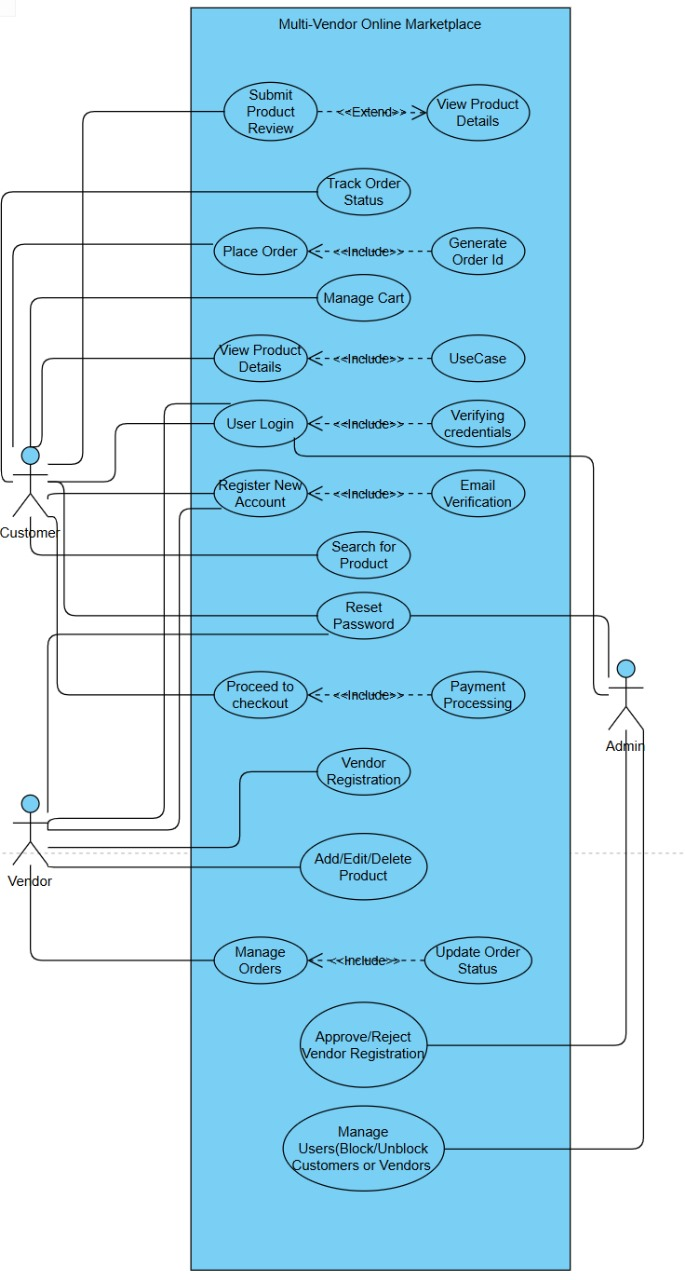
\includegraphics[width=0.9\textwidth]{UseCaseDiagram.jpg}
    \caption{Use Case Diagram for Nexora}
    \label{fig:use-case-diagram}
\end{figure}

\clearpage
\section{Non-Functional Requirements}
The following table outlines the main non-functional requirements for Nexora:

\begin{itemize}
    \item \textbf{Performance}
    \begin{itemize}
        \item NFR-01: The system will handle at least 50 simultaneous users without significant slowdown.
        \item NFR-02: Page load time should not exceed 3 seconds under normal usage conditions.
    \end{itemize}
    \item \textbf{Security}
    \begin{itemize}
        \item NFR-03: User passwords will be securely stored using encryption.
        \item NFR-04: All sensitive data shall be transmitted over HTTPS.
    \end{itemize}
    \item \textbf{Usability}
    \begin{itemize}
        \item NFR-05: The system has a simple and intuitive interface for ease of navigation.
        \item NFR-06: Customers are able to complete a purchase in no more than 5 steps.
    \end{itemize}
    \item \textbf{Scalability}
    \begin{itemize}
        \item NFR-07: The system will allow for future expansion, supporting additional vendors and products.
    \end{itemize}
    \item \textbf{Availability}
    \begin{itemize}
        \item NFR-08: The system maintains an uptime of at least 99\%.
    \end{itemize}
\end{itemize}

\section{Technical Requirements}
\subsection{Frontend}
\begin{itemize}
    \item HTML5, CSS3, JavaScript
    \item Responsive design framework
    \item Modern browser compatibility
    \item Progressive enhancement
\end{itemize}

\subsection{Backend}
\begin{itemize}
    \item Node.js runtime
    \item Express.js framework
    \item RESTful API design
    \item Database integration
\end{itemize}

\subsection{Database}
\begin{itemize}
    \item MySQL database
    \item Data normalization
    \item Indexing strategy
    \item Backup procedures
\end{itemize}

\section{Integration Requirements}
\begin{itemize}
    \item Payment gateway integration
    \item Email service integration
    \item File storage integration
    \item Analytics integration
\end{itemize}

\section{Compliance Requirements}
\begin{itemize}
    \item Data protection regulations
    \item Security standards
    \item Accessibility guidelines
    \item Industry best practices
\end{itemize} 